%\documentclass[useAMS, usenatbib,usegraphicx,letter]{mn2e}
%\documentclass[11pt]{article}
\documentclass[reprint,aps,prd,superscriptaddress,showkeys,showpacs]{revtex4-1}
\usepackage{epsfig,amsmath,natbib}

\usepackage{aas_macros}
\usepackage{amssymb}
\usepackage{amsmath}
\usepackage{dsfont}
\usepackage{hyperref}
\usepackage{color}
\usepackage{pbox}
\usepackage{booktabs}
\usepackage[dvipsnames]{xcolor}

\hypersetup{
	colorlinks=false,
	citecolor=green
}
% \usepackage{graphicx}
% \usepackage{epstopdf}
% \usepackage{natbib}

%%%%%%%%%%%%%%%%%
%Custom commands%
%%%%%%%%%%%%%%%%%

\newcommand{\bb}[1]{\mathbf{#1}}
\newcommand{\bbh}[1]{\mathbf{\hat{#1}}}
\newcommand{\h}[1]{\hat{#1}}

%%%%%%%%%%%%%%%%%%%%%%%%%%%%%%%%%%%%%%%%%%%%%%

\begin{document}

\title{Simulating cosmic variance in Weak Lensing: effects on parameter inferences}

\author{Andrea Petri}
\email{apetri@phys.columbia.edu}
\affiliation{Department of Physics, Columbia University, New York, NY 10027, USA}
\affiliation{Physics Department, Brookhaven National Laboratory, Upton, NY 11973, USA}

\author{Zolt\'an Haiman}
\affiliation{Department of Astronomy, Columbia University, New York, NY 10027, USA}

\author{Morgan May}
\affiliation{Physics Department, Brookhaven National Laboratory, Upton, NY 11973, USA}

\date{\today}

\label{firstpage}

\begin{abstract}

Constraining cosmology using Weak Gravitational Lensing consists in comparing measured feature vectors, of various dimensions $N_b$, with simulated ones. An accurate estimate of the $N_b\times N_b$ feature covariance matrix is essential to obtain accurate parameter confidence intervals. When this covariance matrix $\bb{C}$ is measured from simulations, an important question to ask is how big the simulation set should be for an accurate estimation of $\bb{C}$. We construct different mock ensembles with $N_r$ realizations of the same shear field, using a common randomization procedure based on $N_s<N_r$ independent $N$--body simulations. Previous work \citep{DodelsonSchneider13} showed that noise fluctuations in the feature covariance lead, at quadratic order, to a $O(1/N_r)$ degradation of parameter constraints. Using a variety of features that include shear-shear power spectra and peak counts, we show that cubic and quartic covariance fluctuations lead to additional $O(1/N_r^2)$ error degradation that is not negligible when $N_r$ is only a factor of a few bigger than $N_b$. When we study the large $N_r$ limit we find that a single $N$--body simulation can be recycled a large number of times to produce an ensemble of $N_r=10^5$ shear realizations that are mutually independent. We also find that a small number of independent $N$--body simulations (1 or 2) are necessary to forecast parameter error bars at percent accuracy, while a larger number might be needed to measure accurate feature ensemble means.

\end{abstract}


\keywords{Weak Gravitational Lensing --- Simulations --- Methods: numerical,statistical}
\pacs{98.80.-k, 95.36.+x, 95.30.Sf, 98.62.Sb}

\maketitle


%%%%%%%%%%%%%%%%%%%%%%%%%% INTRO %%%%%%%%%%%%%%%%%%%%%%%%%%%%%%%%%%%%%%%%%%%%%%%%%%%%%%%%

\section{Introduction}
%
Weak Gravitational lensing is a promising cosmological probe for constraining the Dark Energy equation of state $w$, and has been considered by a range of past (CFHTLens \citep{cfht1,cfht2}), current (DES \citep{DES}) and future (LSST \citep{LSST}) experiments. In an era where cosmology is becoming data driven, accurate numerical simulations of shear fields are becoming important for a number of reasons including the study of baryonic effects \citep{BaryonXiuyuan}, non--Gaussian statistics \citep{PeaksJan,MinkJan,MinkPetri} and various systematics. Building cosmological predictions from simulations naturally introduces fluctuations in the forecasts, mainly due to cosmic variance. These fluctuations have been shown to have non negligible effects on estimates of features covariance matrices and hence on parameter constraints (see \citep{DodelsonSchneider13}). This work studies this issue further, focusing on the number of independent $N$--body simulations that is necessary to run for obtaining accurate estimates of parameter constraints, with particular focus on $w$. This paper is organized as follows: in the first paragraph we briefly describe the shear simulation methods we used, as well as the formalism we adopted to compute cosmological parameter constraints. We then outline our main findings and discuss the results, as well as future prospects for continuing this study.  

%%%%%%%%%%%%%%%%%%% METHODS %%%%%%%%%%%%%%%%%%%%%%%%%%%%%%%%%%%%%%%

\section{Methods}

\subsection{Shear field simulations}
\label{shearsim}
%
In this paragraph we describe how we constructed our shear field ensembles. Background galaxies at redshift $z_s$ are lensed by large scale structure between $z=0$ and $z_s$. The shape distortions due to the cosmic shear $\pmb{\gamma}$ can be computed in terms of the dark matter gravitational potential $\Phi(\bb{x},z)$. Because the evolution of $\Phi$ in redshift is non--linear, its evolution needs to be computed with numerical simulations. We make use of the public code \texttt{Gadget2} \citep{Gadget2}, with which we run a sequence of dark--matter--only $N$--body simulations that track the evolution of the density fluctuations in the large scale structure of the universe. We assume a standard $\Lambda$CDM framework with $(\Omega_m,\Omega_\Lambda,h,w,\sigma_8,n_s)=(0.26,0.74,0.72,-1,0.8,0.96)$ and we fix the comoving size of the simulation box to $240\mathrm{Mpc}/h$. We fill the box with $512^3$ particles, which correspond to a mass resolution of $10^{10}M_\odot$. We assume a uniform galaxy distribution at a constant redshift $z_s=2$ (at which the simulation box has an angular size of $\theta_{box}=3.5\mathrm{deg}$) and we discretize the mass distribution between $z_s$ and the observer at $z=0$ with a sequence of 46 two dimensional lenses of thickness $80\mathrm{Mpc}/h$. The surface density on each lens is computed by projecting the three dimensional density measured from \texttt{Gadget2} snapshots. We then apply the multi--lens--plane algorithm (see \citep{RayTracingHartlap,RayTracingJain} for example) to trace the deflections of $n_{ray}^2=2048^2$ light rays arranged on a square grid of total size $\theta_{box}$, from $z=0$ to $z_s$. The light deflection calculations have been performed with our implementation of multi--lens--plane algorithm, which is part of the \texttt{LensTools} computing package \citep{LensTools} (released under the \texttt{MIT} license). Different realizations $r$ of the same shear field $\pmb{\gamma}_r(\pmb{\theta})$ can be generated with different choices of the lenses that lay between the observer and $z_s$. The randomization procedure we adopt is the following:

\begin{itemize}
\item Pick a lens redshift $z_l$, and select the snapshot at $z_l$ from the $i$--th $N$--body simulation at disposal, where $i$ is a random number in $[1,N_s]$
\item Choose randomly a direction between the three choices ${\bb{n}_x,\bb{n}_y,\bb{n}_z}$: the lens plane will be pependicular to this direction
\item Choose the cutting point of the plane in the snapshot: because the lens thickness is 1/3 the size of the box, we can cut three different slices of the simulation box for each orientation ${\bb{n}_x,\bb{n}_y,\bb{n}_z}$, which gives a total of 9 choices for generating a lens plane out of a $N$--body snapshot
\item Perform a periodical random shift of the lens plane along its two directions
\item Repeat this procedure for each lens redshift $z_l$  
\end{itemize}  
%
This randomization procedure allows us to produce an arbitrary number $N_r$ of mock shear realizations $\pmb{\gamma}_r(\pmb{\theta})$, which however will not be all independent if $N_s$ is not large enough. Using a set of 200 independent $N$--body simulations, we construct different ensembles with different choices of $N_s\in[1,200]$, each made of 1000 mock shear realizations. We also build an additional ensemble with $N_s=1$ and $10^5$ mocks. From each of these mocks we reconstruct the convergence $\kappa_r(\pmb{\theta})$ and measure its angular power spectrum $P^{\kappa\kappa}_r(l)$ defined as
\begin{equation}
\langle\tilde{\kappa}_r(\bb{l})\tilde{\kappa}_r(\bb{l}')\rangle = (2\pi)^2\delta_D(\bb{l}+\bb{l}')P^{\kappa\kappa}_r(l)
\end{equation}
%
As an additional summary statistic, we consider the counts of local $\kappa$ maxima of a certain height $\kappa_0$, $n_r(\kappa_0)$ (from now on \textit{peak counts}), with varying $\kappa_0$. The fact that the ensemble of $N_r$ mocks is not completely independent if $N_s$ is not large enough can have an effect on the covariance estimators of $P^{\kappa\kappa},n(\kappa_0)$. 


\subsection{Parameter inference}
%
Let $\bbh{d}$ a feature of dimension $N_b$, $\bb{d}(\bb{p})$ be the smooth expectation of this feature at a point $\bb{p}$ in parameter space (which has a dimension $N_p$) and $\bb{C}$ be the $N_b\times N_b$ feature covariance matrix. For the purpose of this work $\bb{p}$ is the triplet $(\Omega_m,w,\sigma_8)$ and $\bb{d}$ is one of the features listed in Table \ref{featuretable}. While, in some cases, $d(\bb{p})$ can usually be predicted reasonably accurately by already existing emulators (see \citep{coyote2,Nicaea} for example), the matter is more complicated for covariance matrices. Estimating $\bb{C}$ from simulations involves generating a series of mock realizations $\bbh{d}_r$ with $r=1...N_r$ and estimating the sample covariance $\bbh{C}$

\begin{equation}
\bb{\bar{d}} = \frac{1}{N_r}\sum_{r=1}^{N_r} \bbh{d}_r
\end{equation}

\begin{equation}
\label{covest}
\bbh{C} = \frac{1}{N_r-1}\sum_{r=1}^{N_r} (\bbh{d}_r - \bar{\bb{d}}) (\bbh{d}_r - \bar{\bb{d}})^T
\end{equation}
%
Assuming a normal feature likelihood, together with a flat prior on the parameter space, the parameter posterior distribution $\mathcal{L}(\bb{p}\vert\bbh{d}_{obs})$ given an observed instance of $\bbh{d}$, which we call $\bbh{d}_{obs}$, can be obtained using Bayes theorem
\begin{equation}
\label{posteriorbayes}
-2\log\mathcal{L}(\bb{p}\vert\bbh{d}_{obs}) = (\bbh{d}_{obs}-\bb{d}(\bb{p}))^T\bbh{C}^{-1}(\bbh{d}_{obs}-\bb{d}(\bb{p}))
\end{equation}
%
For the sake of simplicity, we approximate the posterior as a Gaussian around its maximum. This is easily done approximating the simulated feature at first order around a point $\bb{p}_0$ (that ideally is the maximum of (\ref{posteriorbayes}))
\begin{equation}
\bb{d}(\bb{p}) \approx \bb{d}_0 + \bb{d}_0^\prime(\bb{p}-\bb{p}_0) 
\end{equation}
%
To measure the feature derivatives $\bb{d}'_0$ with respect to cosmology, we make use of the public code \texttt{NICAEA} \citep{Nicaea} for the power spectrum, and we use an independent simulation set (that contains mocks at different combinations of $(\Omega_m,w,\sigma_8)$, see Table \ref{simtable}) for the peak counts.

\begin{table}
\begin{center}
\begin{tabular}{c|c|c||c|c}
\toprule
$\Omega_m$ &  $w$ & $\sigma_8$ & $N_s$ & Number of $\kappa$ ensembles \\ \hline \hline
\midrule

0.26 & -1 & 0.8 & $1\div 200$ & 16 \\
0.29 & -1 & 0.8 & 1 & 1 \\
0.26 & -0.8 & 0.8 & 1 & 1 \\
0.26 & -1 & 0.6 & 1 & 1 \\

\bottomrule
\end{tabular}
\end{center}
\caption{Summary table of the shear ensembles used in this work.}
\label{simtable}
\end{table}

We can build the estimator for the posterior maximum $\bbh{p}$, given the observation $\bbh{d}_{obs}$, as follows:
%
\begin{equation}
\label{estimatormean}
\bbh{p} = \bb{p}_0 + \bbh{T}(\bbh{d}_{obs}-\bb{d}_0)
\end{equation}

\begin{equation}
\bbh{T} = (\bb{d}_0'^T\bbh{C}^{-1}\bb{d}_0')^{-1}\bb{d}_0'^T\bbh{C}^{-1}
\end{equation}
%
Because $\bbh{p}$ is estimated using a noisy data instance $\bbh{d}_{obs}$, its estimate will be scattered around the true value $\langle\bbh{p}\rangle_O$. In the following we use the $\langle\rangle_O$ notation for expectation values taken with respect to observations, while we keep the notation $\langle\rangle$ for expectation values taken with respect to the simulations. Defining the \textit{precision matrix} $\bbh{\Psi}=\bbh{C}^{-1}$, we can express the estimator of the observational scatter in $\bbh{p}$

\begin{equation}
\label{estimatorcovariance}
\h{\Sigma}_\bb{p} = \bbh{F}^{-1}\bb{d}_0'^T\bbh{\Psi}\langle(\bbh{d}_{obs}-\bb{d}_0)(\bbh{d}_{obs}-\bb{d}_0)^T\rangle_O\bbh{\Psi}\bb{d}_0'\bbh{F}^{-1}
\end{equation}

\begin{equation}
\label{estimatorfisher}
\bbh{F} = \bb{d}_0'^T\bbh{\Psi}\bb{d}_0'
\end{equation}
%
Where we introduced the Fisher matrix estimator $\bbh{F} = \bb{d}_0'^T\bbh{\Psi}\bb{d}_0'$ and, for simplicity, we assumed $\langle\bbh{d}_{obs}\rangle_O=\bb{d}_0$, so that $\langle(\bbh{d}_{obs}-\bb{d}_0)(\bbh{d}_{obs}-\bb{d}_0)^T\rangle_O=\bb{C}$. 
When we perform an observation $\bbh{d}_{obs}$, the parameter estimate $\bbh{p}$ is a random draw from a probability distribution with variance $\h{\Sigma}_\bb{p}$, which inherits noise from the simulations. The noise in the covariance estimator (\ref{covest}) and its inverse $\bbh{\Psi}$ propagates all the way to the posterior (\ref{posteriorbayes}), the parameter estimate (\ref{estimatormean}) and its variance (\ref{estimatorcovariance}). Following \citep{DodelsonSchneider13,Taylor12,MasumotoWishart} we compute the expectation value of (\ref{estimatorcovariance}) over simulations, $\langle\h{\Sigma}_\bb{p}\rangle$, up to $O(1/N_r^2)$ by expanding (\ref{estimatorcovariance}) to quartic order in the $\bbh{\Psi}$ statistical fluctuations. Indicating the noiseless parameter covariance as $\Sigma_\bb{p}=\bb{F}^{-1}$, the result we get is \footnote{The details of the calculation are given in Appendix A}  

\begin{widetext}
\begin{equation}
\label{quarticdegradation}
\langle\h{\Sigma}_\bb{p}\rangle = \Sigma_\bb{p}\left[1+\frac{N_b-N_p}{N_r}+\frac{(N_b-N_p)(N_b-N_p+2)}{N_r^2}\right] + O\left(\frac{1}{N_r^3}\right)
\end{equation}
\end{widetext}
%
Next, we restrict ourselves to the large $N_r$ limit, and we further investigate the behavior of the $O(1/N_r)$ term. We consider three cases \footnote{The details of these calculations are given in Appendix B}:
\begin{enumerate}
\item If the true data covariance $\bb{C}$ is known, the estimator (\ref{estimatorcovariance}) is biased, and the dominant contribution of the bias comes from the second order fluctuations in $\bbh{\Psi}$. Once the expectation values over simulations are taken, the bias sums up to 

\begin{equation}
\label{dodelsonscaling}
\langle\h{\Sigma}_\bb{p}\rangle=\Sigma_\bb{p}\left(1+\frac{N_b-N_p}{N_r}\right)
\end{equation}
%
This is the result obtained by \citep{DodelsonSchneider13}.

\item Usually the true covariance is not known, and it is tempting to plug in its estimator $\bbh{C}$, measured from the same simulation set we use to compute $\bbh{\Psi}$. This approach has been used before in the literature (see \citep{MinkPetri,MinkShirasaki} for example). If we do that, and we do not correct for the $\bbh{\Psi}$ bias (see equation (\ref{firstmoment})), the parameter variance will have a contribution from both the second and first order fluctuations in $\bbh{\Psi}$, which now have a non zero expectation value. In this case the bias sums up to 
\begin{equation}
\label{mockscalinguncorrected}
\langle\h{\Sigma}_\bb{p}\rangle=\Sigma_\bb{p}\left(1-\frac{N_b-N_p}{N_r}\right)
\end{equation}

\item If we repeat the same exercise as above, but we correct for the bias in the precision matrix estimator, we are left with 

\begin{equation}
\label{mockscalingcorrected}
\langle\h{\Sigma}_\bb{p}\rangle=\Sigma_\bb{p}\left(1+\frac{1+N_p}{N_r}\right)
\end{equation}

\end{enumerate} 
%
The error degradation  in each parameter $p$, at dominant order, scales as $D/N_r$, where $D=N_b-N_p,N_p-N_b,1+N_p$ for cases 1,2,3 respectively. This means that, when parameter errors are estimated purely from simulations, and the same simulation set is used to estimate both $\bbh{C},\bbh{\Psi}$, these errors tend to decrease with $N_b$ (case 2), or at best remain constant (case 3), while the distribution of $\bbh{p}$ has still a variance that increases with $N_b$. This typically leads to underestimates in parameter errors. We test the scaling relation
\begin{equation}
\label{ourscaling}
\langle\h{\sigma}_p^2\rangle = \sigma^2_{p,\infty}(N_s)\left(1+\frac{D}{N_r}\right)
\end{equation}
%
on our simulations for high and small $N_r$. We use notation $\h{\sigma}^2_p=\h{\Sigma}_{pp}$ and we indicate as $\sigma^2_{p,\infty}$ the expectation value of the variance in the limit of infinite mocks $N_r\rightarrow\infty$. We call $D$ the \textit{effective dimensionality} of the feature space (which, as seen before, can be negative in some cases). We compute the expectation values of $\h{\sigma}^2_p$ (equations (\ref{estimatorcovariance}),(\ref{ourscaling})) averaging over 100 random resamplings of our shear ensembles. For the true feature covariance matrix $\langle(\bbh{d}-\bb{d}_0)(\bbh{d}-\bb{d}_0)^T\rangle=\bb{C}$ we use the estimated covariance from a grand ensemble built with the union of all the ensembles with different $N_s$. 

The true parameter variance $\sigma^2_{p,\infty}(N_s)$ in principle depends on the number of independent $N$--body simulations $N_s$, which appears in the randomization procedure we describe in \S~\ref{shearsim}. The reason for this can be found in that, if $N_s$ is not big enough, the different shear realizations cannot be all independent, and hence the true variance $\sigma^2_{p,\infty}(N_s\rightarrow\infty)$ cannot be recovered for low $N_s$ even if $N_r$ is large. In the next paragraph we outline our main findings.
 

%%%%%%%%%%%%%%%%%%% RESULTS %%%%%%%%%%%%%%%%%%%%%%%%%%%%%%%%%%%%%%%

\section{Results} 

%%%%%%%%%%%%%%%%%%%%%%%%%%%%%%%%%%%%%%%%%%%%%%%%%%%%%%%%%%%%%%%%%%%%%%

\begin{figure*}
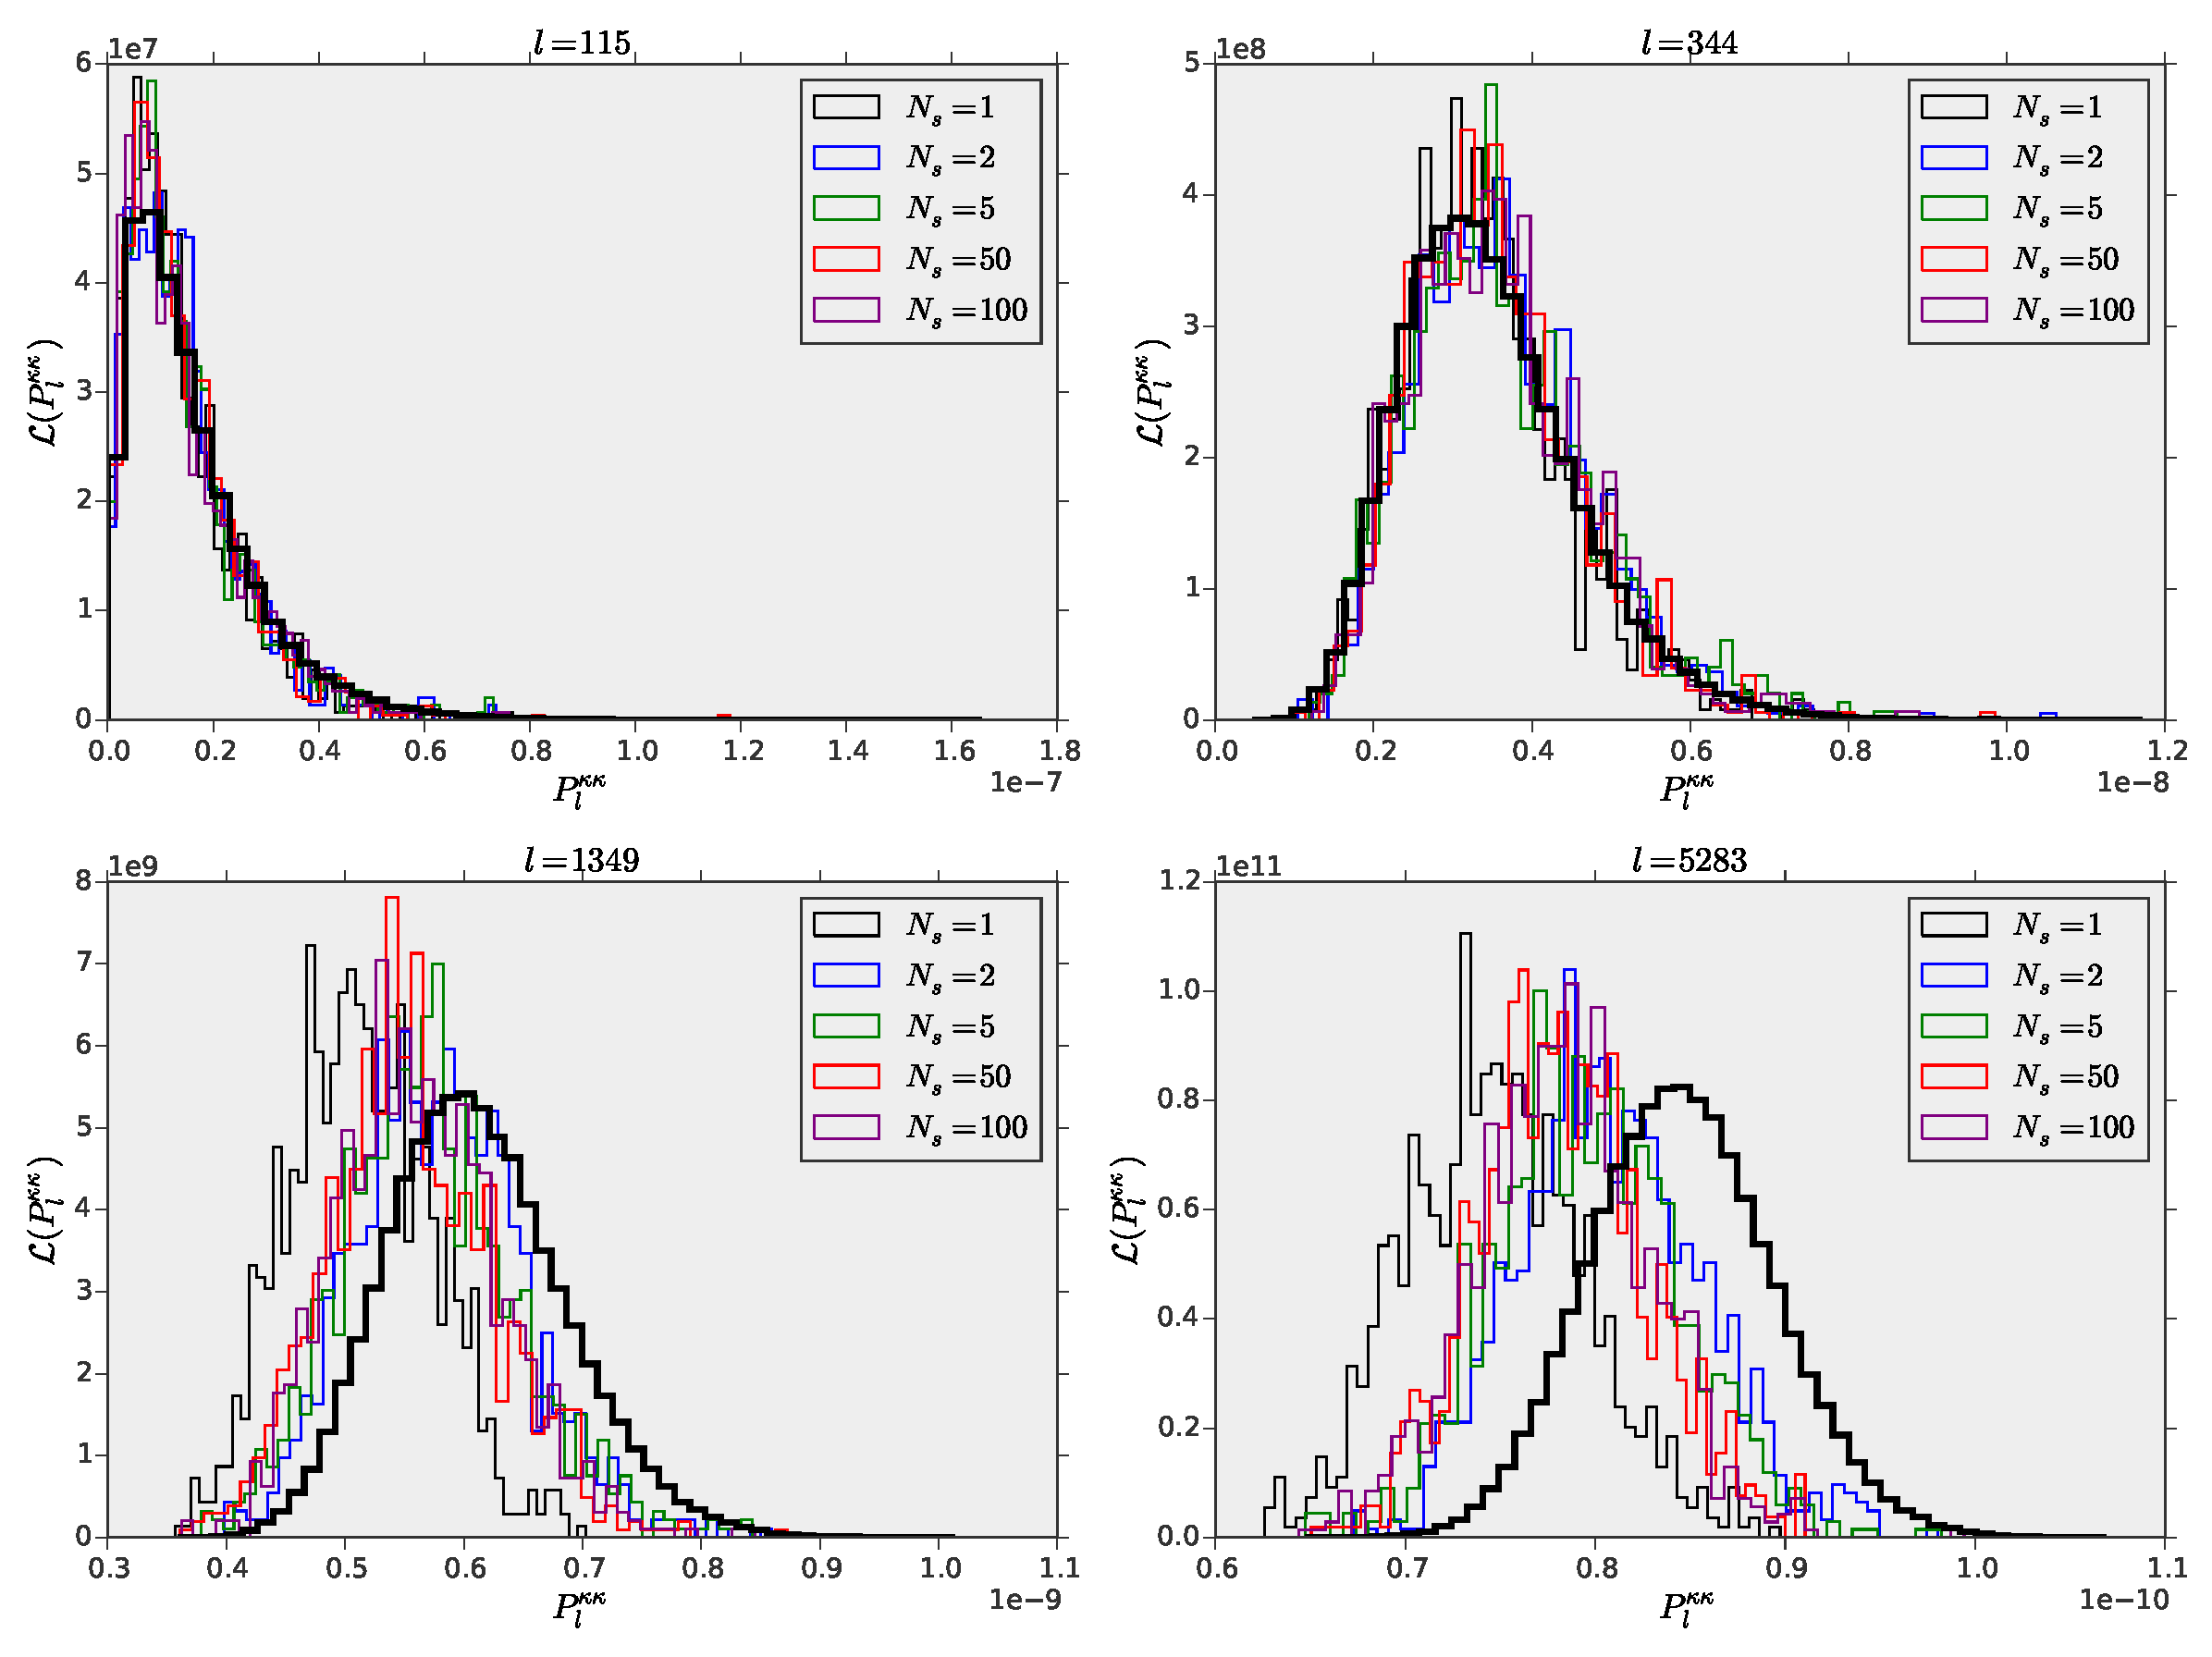
\includegraphics[scale=0.4]{Figures/ps_pdf.eps}
\caption{PDF of the $\kappa$ power spectrum,$\mathcal{L}(P_l^{\kappa\kappa})$, at four selected multipoles $l=115,344,1349,5283$, for different shear ensembles constructed with $N_s=$1 (black), 2 (blue), 5 (green), 50 (red), 100 (purple). The thick black lines correspond to an ensemble generated with $N_s=1$ and $10^5$ mock realizations.}
\label{ps_pdf}
\end{figure*}

\begin{figure}
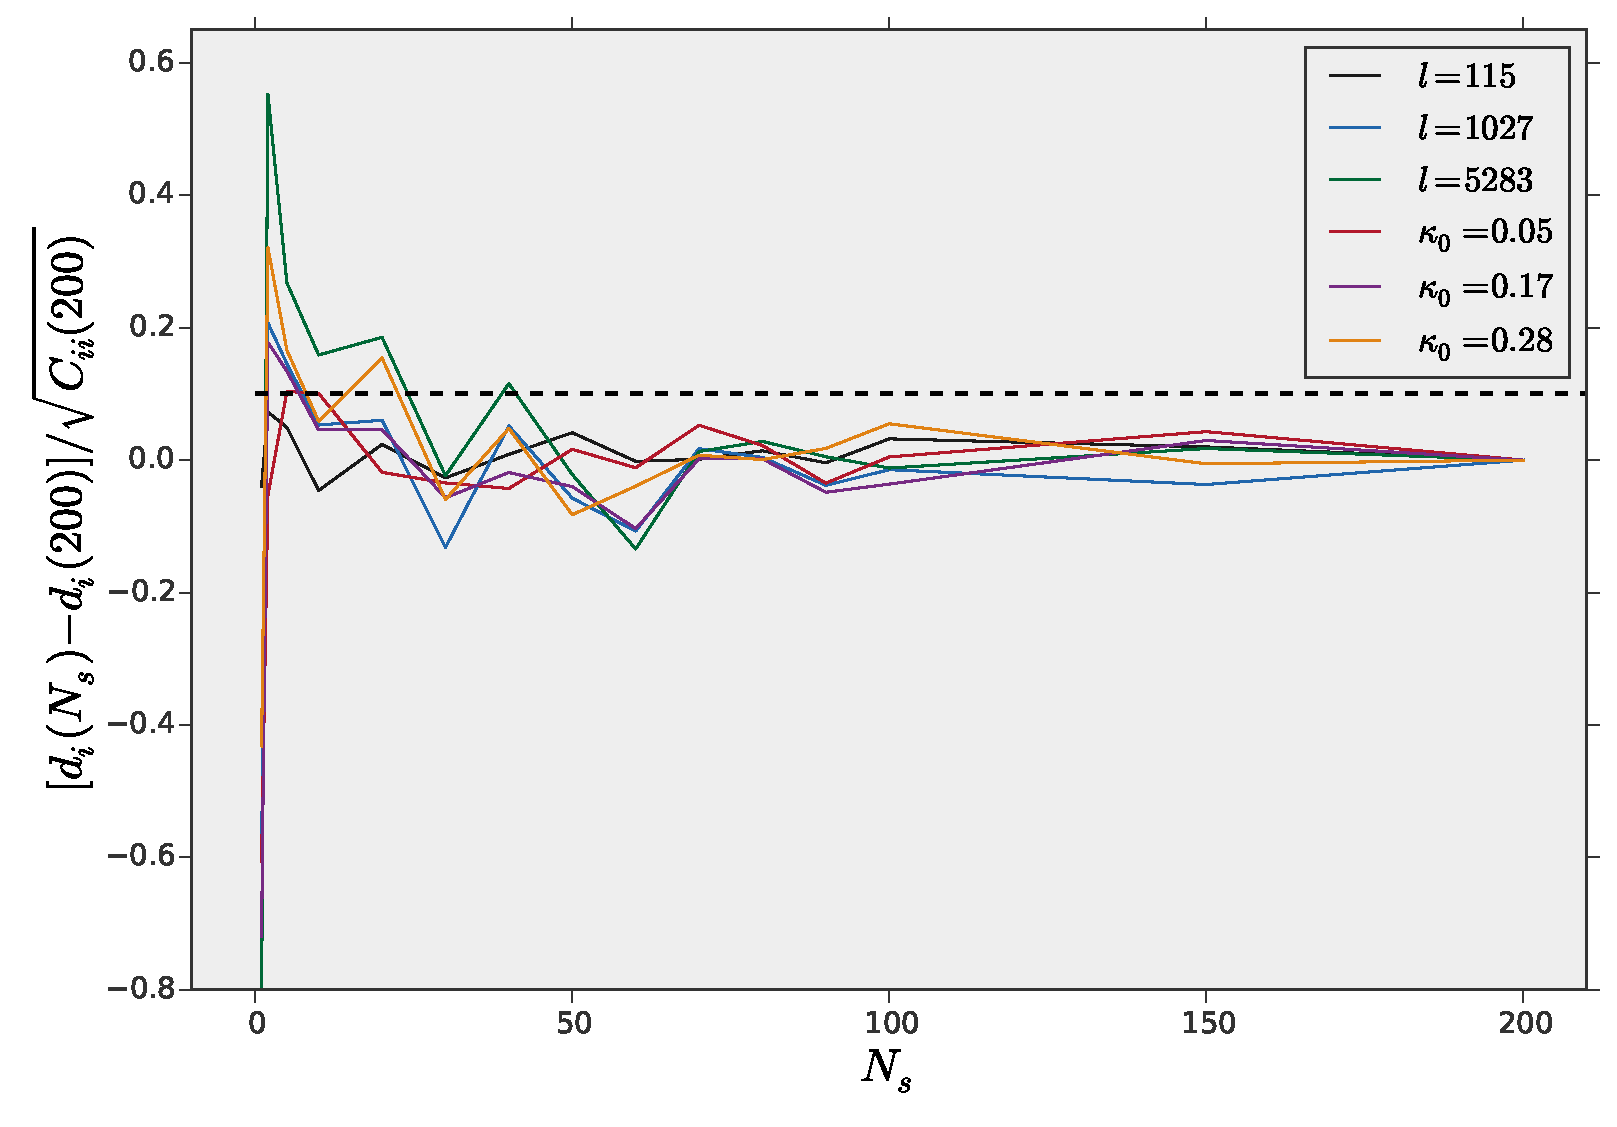
\includegraphics[scale=0.3]{Figures/means_ns.eps}
\caption{Means of shear features $d$ measured from different shear ensembles. The quantities shown are the differences between mean features measured from ensemble with varying $N_s$, with respect to the means measured from the $N_s=200$ ensemble, in units of the statistical error measured from the $N_s=200$ ensemble. The colored lines refer to shear-shear power spectra measured at $l=115$ (black), 1027 (cyan), 5283 (green) and peak counts of height $\kappa_0=0.05$ (red), 0.17 (purple), 0.28 (orange).}
\label{means_ns}
\end{figure}

\begin{figure}
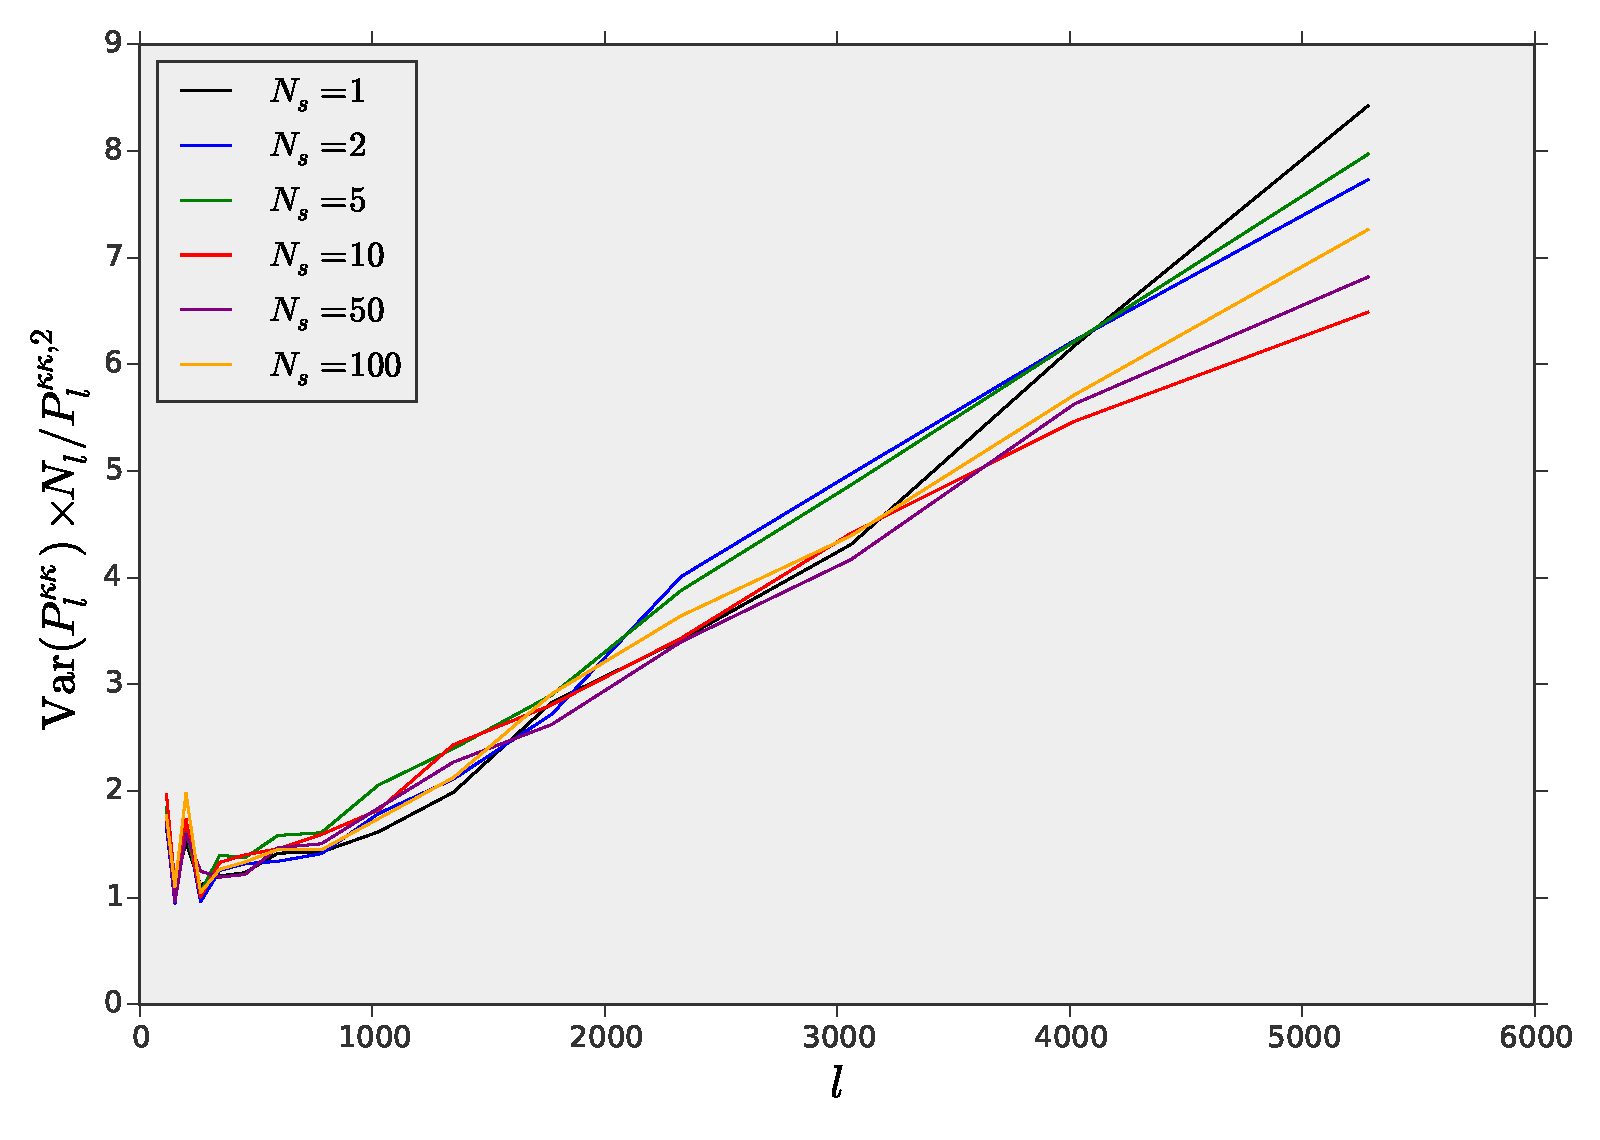
\includegraphics[scale=0.3]{Figures/ps_variance.eps}
\caption{Variance of the $\kappa$ power spectrum as a function of the multipole $l$, in units of the expected gaussian variance from equation (\ref{gaussianvar}). The variance is measured from different shear ensembles with $N_s=$1 (black), 2 (blue), 5 (green), 10 (red), 50 (purple), 100 (orange). }
\label{ps_var}
\end{figure}

\begin{figure}
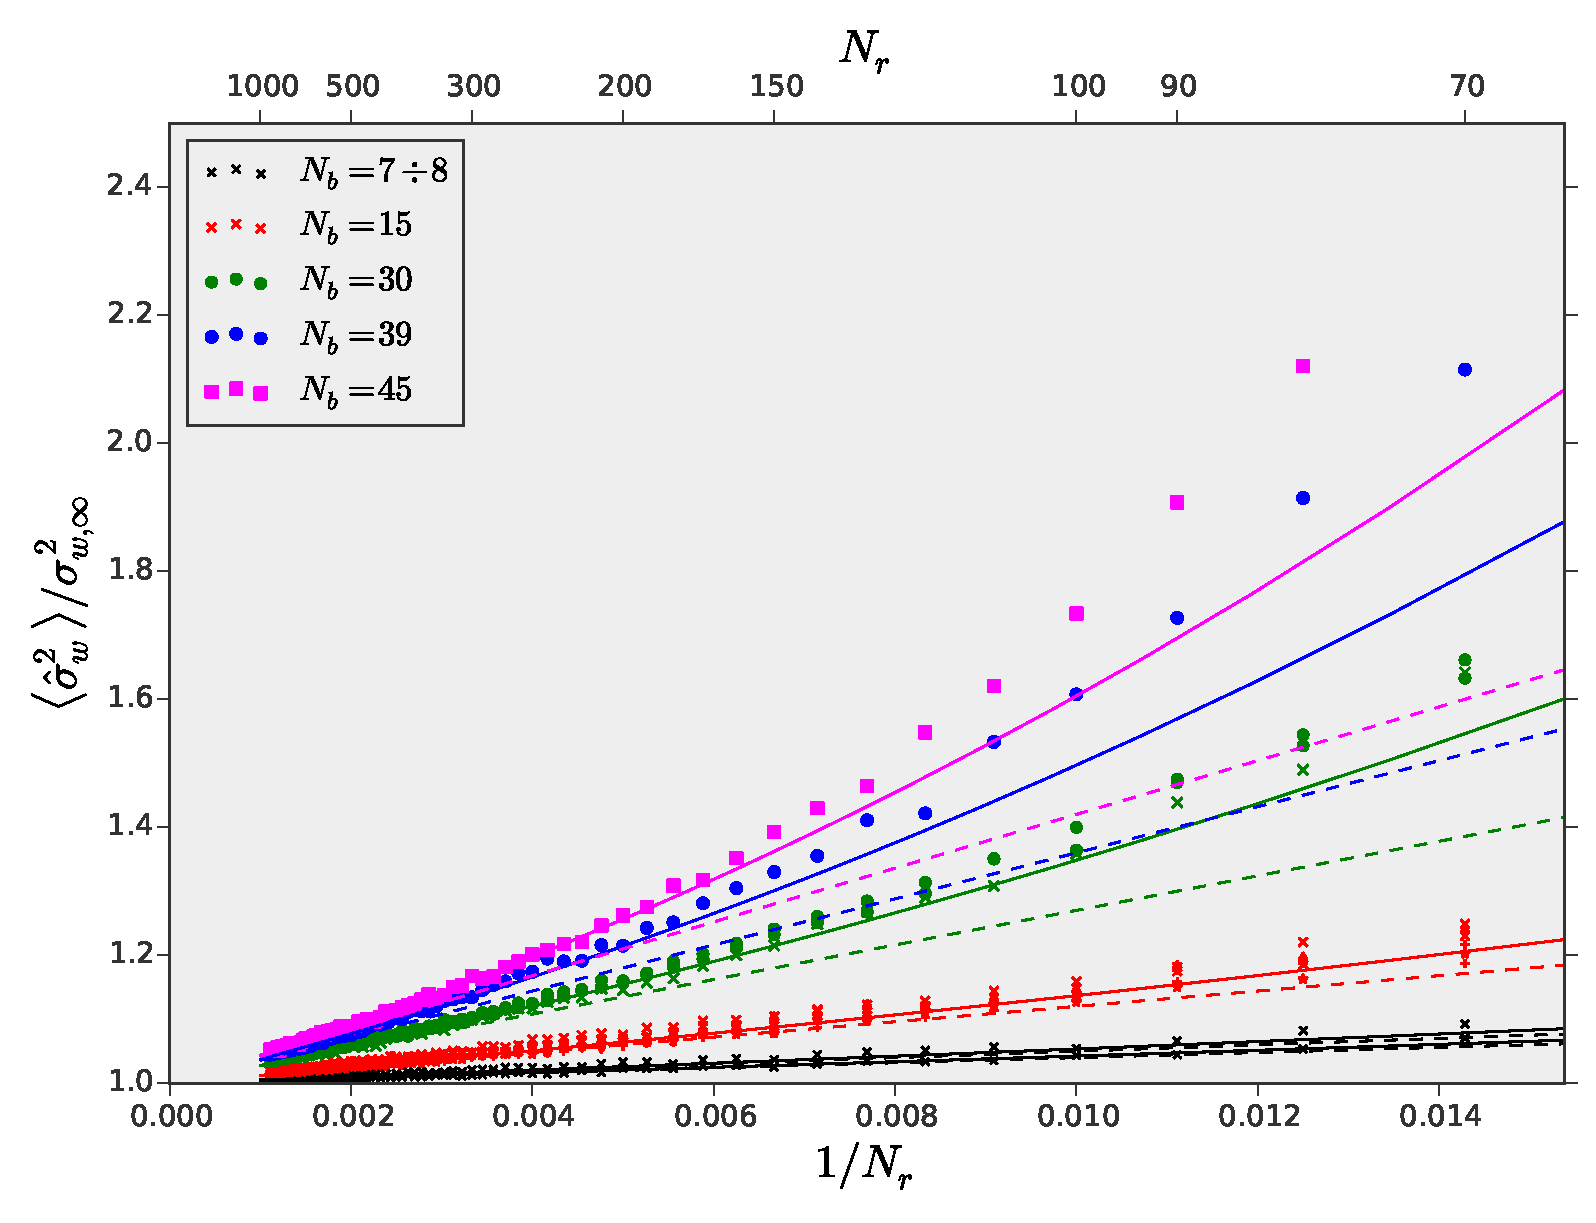
\includegraphics[scale=0.3]{Figures/curving_nb.eps}
\caption{Expectation value of the $w$ variance computed with equation (\ref{estimatorcovariance}) as a function of $1/N_r$, for the features outlined in Table \ref{featuretable}. The dashed and solid lines show the the theory predictions from equation (\ref{quarticdegradation}) at orders $O(1/N_r),O(1/N_r^2)$. The asymptotic variance $\sigma^2_{w,\infty}$ has been computed from a linear regression of $\langle\h{\sigma}^2_w\rangle$ vs $1/N_r$ for $N_r>500$.}
\label{curvingnb}
\end{figure}

\begin{figure}
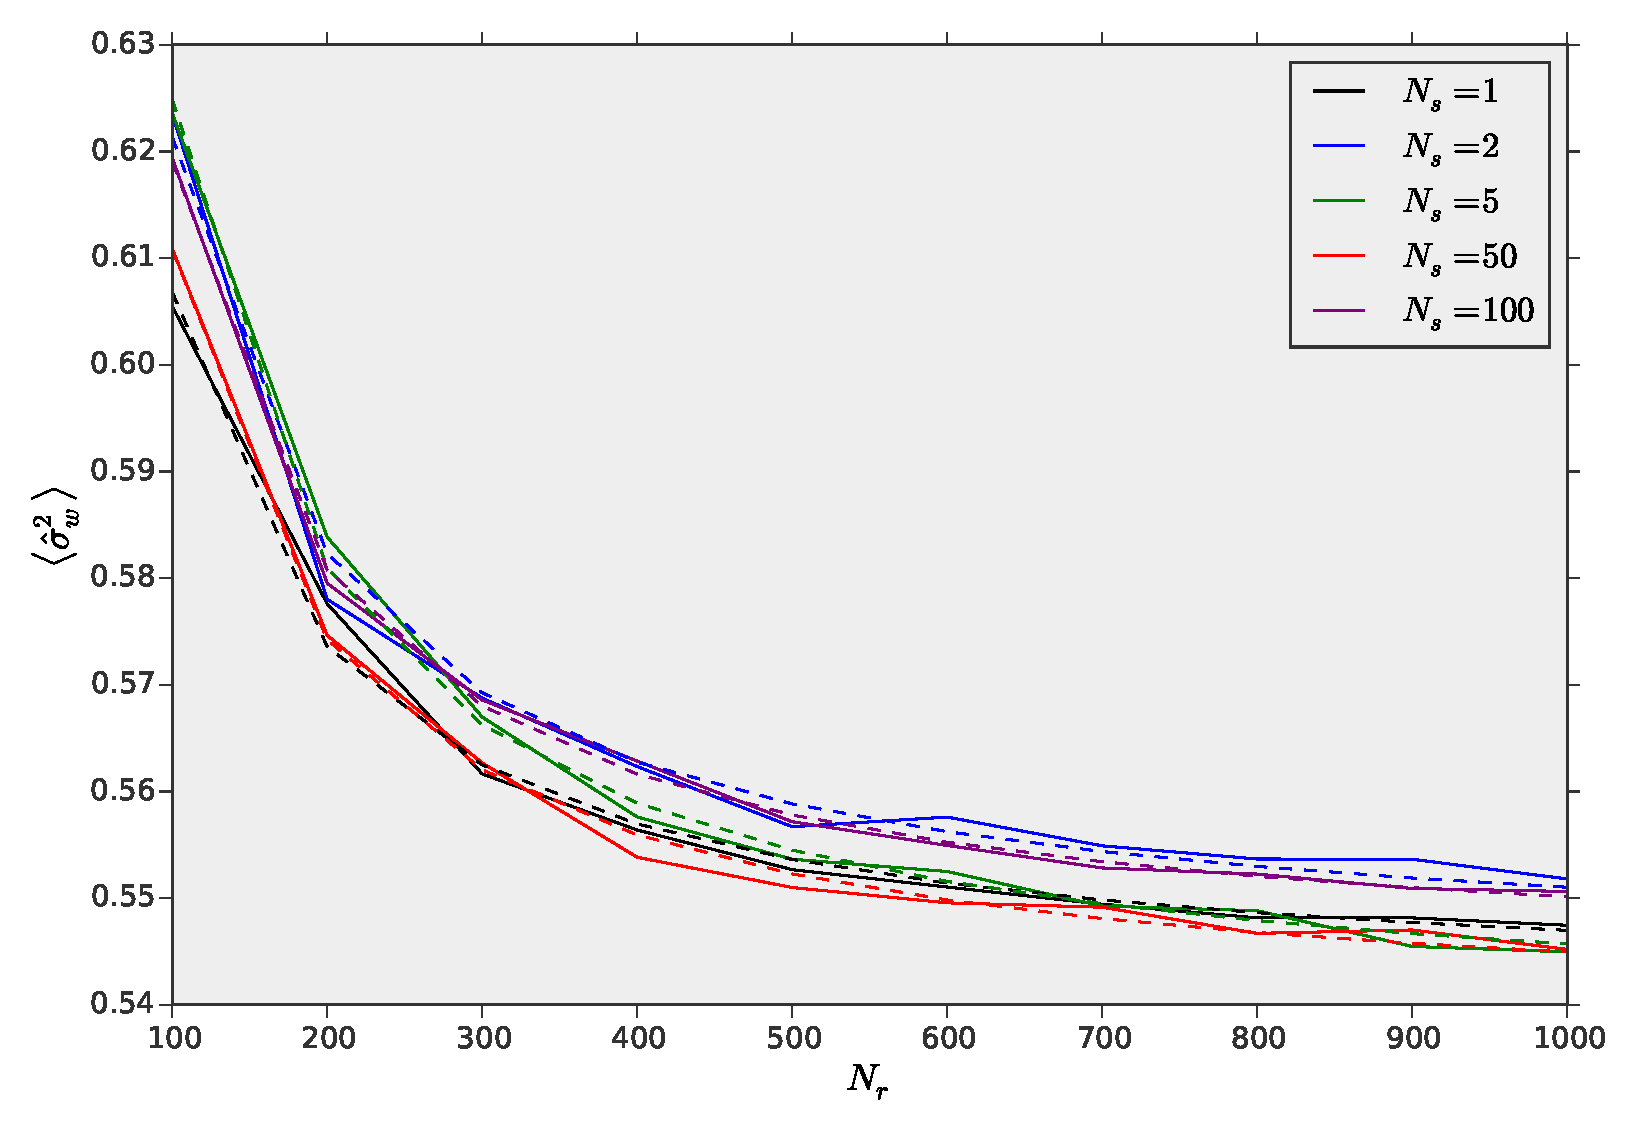
\includegraphics[scale=0.3]{Figures/scaling_nr.eps}
\caption{Bias in the $w$ variance, $\langle\h{\sigma}^2_w\rangle-\sigma^2_{w,\infty}$, as a function of the number of mock realizations $N_r$ used in the feature covariance estimator (\ref{covest}). Results for different mock ensembles generated with $N_s=$1 (black), 2 (blue), 5 (green), 50 (red), 100 (purple) are shown. The figure shows both the measured trends (solid lines) and their best fits according to equation (\ref{ourscaling}). The thick black line correspond to an ensemble generated with $N_s=1$ and $10^5$ mock realizations. }
\label{wvar_nr}
\end{figure}

\begin{figure}
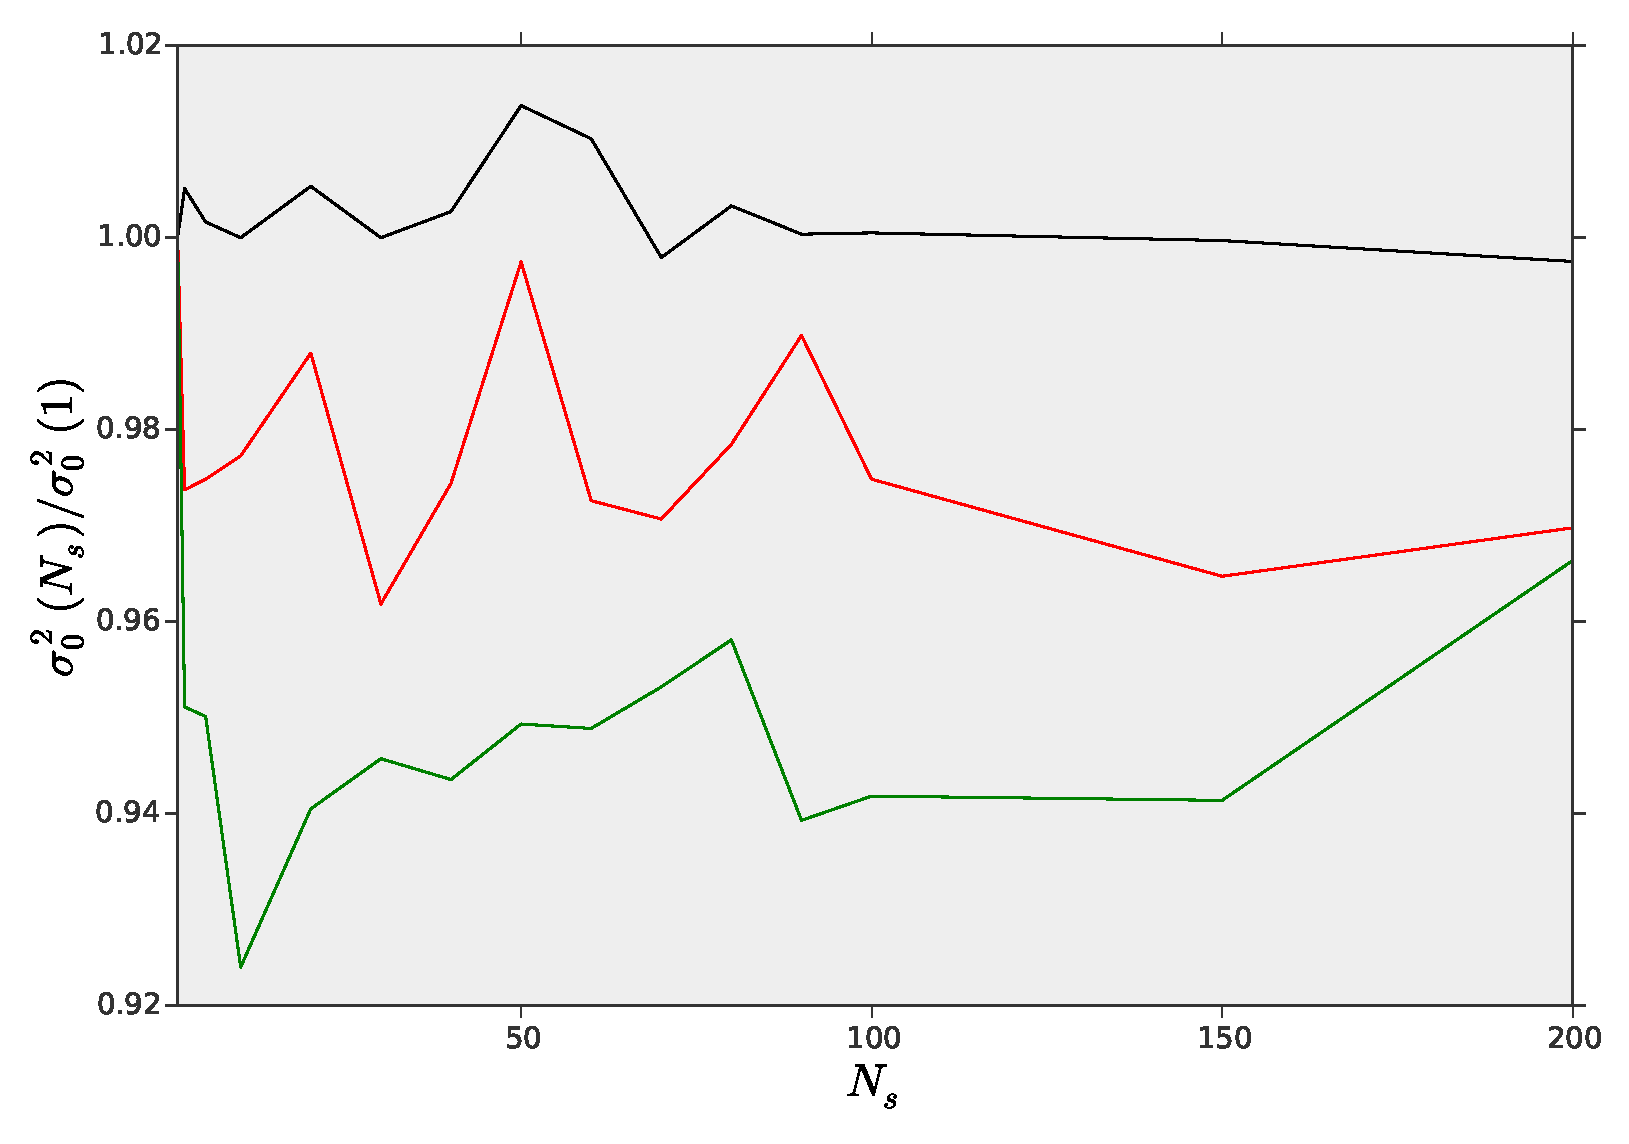
\includegraphics[scale=0.3]{Figures/scaling_ns.eps}
\caption{Variance on $w$ in the limit $N_r\rightarrow\infty$, varying the mock ensemble used to compute the covariance estimator (\ref{covest}). We show the dependence of $\sigma_{w,\infty}^2(N_s)$ in units of the mean over $N_s$, for the power spectrum logarithmically binned (black), the power spectrum linearly binned (red) and the peak counts (green).}
\label{wvar_ns}
\end{figure}

\begin{table*}
\begin{center}
\begin{tabular}{ccccc}
\toprule
\textbf{Feature} &  \textbf{Specifications} & $N_b$ &  \textbf{Symbol} & \textbf{Color} \\ \hline \hline
\midrule
Power Spectrum, log binning  & $l \in [100,800] $ & 8 & $\times$ & black  \\ 
Power Spectrum, log binning  & $l \in [1000,6000] $ & 7 & $\blacksquare$ & black  \\ 
Power Spectrum, log binning  & $l \in [100,6000] $ & 15 & \textcolor{red}{$\bullet$} & \textcolor{red}{red}  \\
Power Spectrum, linear binning  & $l \in [100,2000] $ & 15 & \textcolor{red}{$+$} & \textcolor{red}{red}  \\ 
Power Spectrum, linear binning  & $l \in [2500,4500] $ & 15 & \textcolor{red}{$\times$} & \textcolor{red}{red}  \\
Power Spectrum, linear binning  & $l \in [100,4500] $ & 30 & \textcolor{OliveGreen}{$\bullet$} & \textcolor{OliveGreen}{green}  \\ 
Power Spectrum, linear binning  & $l \in [100,6000] $ & 39 & \textcolor{blue}{$\bullet$} & \textcolor{blue}{blue}  \\ \hline
Low peaks  & $\kappa_0 \in [-0.06,0.09] $ & 15 & \textcolor{red}{$+$} & \textcolor{red}{red}  \\ 
Intermediate peaks  & $\kappa_0 \in [0.1,0.27] $ & 15 & \textcolor{red}{$\bigstar$} & \textcolor{red}{red}  \\ 
High peaks  & $\kappa_0 \in [0.28,0.45] $ & 15 & \textcolor{red}{$\diamond$} & \textcolor{red}{red}  \\
Low+Intermediate peaks  & $\kappa_0 \in [-0.06,0.27] $ & 30 & \textcolor{OliveGreen}{$\times$} & \textcolor{OliveGreen}{green}  \\
Intermediate+High peaks  & $\kappa_0 \in [0.1,0.45] $ & 30 & \textcolor{OliveGreen}{$\blacksquare$} & \textcolor{OliveGreen}{green}  \\
All peaks  & $\kappa_0 \in [-0.06,0.45] $ & 45 & \textcolor{magenta}{$\blacksquare$} & \textcolor{magenta}{magenta}  \\ \hline
\bottomrule
\end{tabular}
\end{center}
\caption{Catalog of feature types used in this work, along with the chosen number of bands $N_b$ and the plot legends for Figure \ref{curvingnb}.}
\label{featuretable}
\end{table*}

%%%%%%%%%%%%%%%%%%%%%%%%%%%%%%%%%%%%%%%%%%%%%%%%%%%%%%%%%%%%%%%%%%%%%%

In this section we outline the main results of this work. We show the qualitative behavior of a variety of features $\bbh{d}_r$ probability distribution function (PDF) in ensembles built with different $N_s$. Figure \ref{ps_pdf} shows the power spectrum PDF at four selected multipoles, Figure \ref{means_ns} shows the dependence of feature ensemble means on $N_s$, while Figure \ref{ps_var} shows the variance in each measure power spectrum multipole. This last result is compared to the one that would be obtained assuming that the convergence $\kappa$ is a Gaussian random field
\begin{equation}
\label{gaussianvar}
\mathrm{Var}(P^{\kappa\kappa}(l)) = \frac{P^{\kappa\kappa,2}(l)}{N_{eff}(l)}
\end{equation}
%
where $N_{eff}(l)$ is the number of independent modes used to estimate the power spectrum at $l$. To measure $P^{\kappa\kappa}(l),N_{eff}(l)$, we compute the real Fourier transform of the pixelized map $\kappa_r(\pmb{\theta})$ with the FFT algorithm. Each Fourier pixel $(i_x,j_y)$ corresponds to a mode $(l_x,l_y)=2\pi(i_x,i_y)/\theta_{box}$, with $i_x=-n_{ray}/2,...,n_{ray}/2$ and $i_y=0,...,n_{ray}/2$. We count the number of pixels $N(l)$ that fall inside a multipole bin $(l_1,l_2)$. Because the $\kappa$ field is real, the modes $(\pm l_x,0)$ are not independent. If we let $N(l,l_y=0)$ be the number of non--independent modes, the mode counting for the variance should be corrected as 

\begin{equation}
N_{eff}(l) = \frac{N^2(l)}{N(l)+N(l,l_y=0)}
\end{equation}
%
We not that this correction is important at low $l$ only, where pixelization effects are more important. In other words $N_{eff}(l\gg2\pi/\theta_{box})\approx N(l)$. 

Figure \ref{curvingnb} shows a comparison between the dependence of $\langle\h{\sigma^2_w}\rangle$ measured from simulations and the theory prediction from equation (\ref{quarticdegradation}). 

Figure \ref{wvar_nr} shows the scaling of the expectation value of $\h{\sigma}_w^2$ when the number of mocks is large, $N_r\gg500$, using the power spectrum and compare it with the known result obtained in \citep{DodelsonSchneider13} and expressed in equation (\ref{ourscaling}). Finally, Figure \ref{wvar_ns} shows the effect of varying $N_s$ on the $w$ constraint.  

%%%%%%%%%%%%%%%%%% DISCUSSION %%%%%%%%%%%%%%%%%%%%%%%%%%%%%%%%%%%%%

\section{Discussion}

In this section we discuss our main findings. Figure \ref{ps_pdf} shows that, although different choices of $N_s$ do not seem to affect the power spectrum PDF at large scales (top two panels), there are some qualitative differences on small scales (bottom two panels), on which a shear ensemble built with a small $N_s$ does not have the same statistical behavior of ensembles built with large $N_s$. Looking at the black curves, we see that the $N_s=1$ ensembles exibit some stochastic fluctuations in where the PDF peaks. We need as small as $N_s=2$ to recover the right location parameter for the power spectrum on small scales. Figure \ref{means_ns} shows that mutiple independent $N$--body simulations $N_s>1$ are necessary for measuring the means of feature ensembles to an accuracy corresponding to 10\% of the statistical error. The number of required simulations $N_s$ depends on the feature type and ranges from a few (1 or 2) for the power spectrum at small multipoles $l\lesssim 500$ to an order of $30\div50$ for the power spectrum at large multipoles $l\gtrsim1000$ peak counts at a high threshold $\kappa_0\approx0.3$.   

Figure \ref{ps_var} shows the variance of convergence power spectrum computed from different ensembles, in units of the Gaussian expectation. We find that, even with $N_s=1$, our results are in good agreement with the ones obtained by \citep{Sato12}, which used $N_s=400$. This fact by itself is not sufficient to conclude that $N_s$ does not have an effect on parameter inferences, since these depend on the cross band covariances.

Figure \ref{curvingnb} shows that error degradation estimates truncated at order $O(1/N_r)$ are too optimistic when the number of mocks $N_r$ used to measure the covariance is only a factor of few larger than the dimension of the feature space $N_b$. In these cases effects coming the next--to--leading orders $O(1/N_r^2)$ become non--negligible on constraints degradation. In particular we find that already for $N_b=30$ and $N_r\sim100$, error degradation estimates at $O(1/N_r^2)$ are too optimistic, and more accurate estimates require at least the terms of order $O(1/N_r^3)$, which come from higher than quartic $\bbh{\Psi}$ fluctations.      

In Figure \ref{wvar_nr} we examine how the $w$ constraint depends on the number of mocks used to estimate the covariance in the limit of large $N_r$, and we find good agreement with (\ref{ourscaling}) up to values comparable to $\sim 10^5$. Bacause of this, we can argue that one $N$--body simulation is enough to construct an ensemble of $O(10^5)$ mutually independent mock power spectra.    

Figure \ref{wvar_ns} shows the dependence of the dark energy constraint with $N_s$. We find that, in the range $N_s\in[1,200]$ the $w$ inferred variance $\sigma_{w,\infty}^2$ fluctuates stochastically and does not show an appreciable trend with $N_s$. 

When we estimate the data covariance $\bb{C}$ from the same simulation set used to measure $\bbh{\Psi}$, the effective dimensionality $D$ decreases with increasing $N_b$ in the case where the $\bbh{\Psi}$ bias is corrected, and stays constant when this bias is corrected. This fact that should be taken into considerations when estimating parameter errors purely from simulations, as underestimations might occur. 

%%%%%%%%%%%%%%%%%% CONCLUSION %%%%%%%%%%%%%%%%%%%%%%%%%%%%%%%%%%%%%

\section{Conclusion}

In this work we examine the effect of $N$--body simulations based shear ensembles on forecasted cosmological constraints. Our main results can be summarized as follows:

\begin{itemize}
\item When the feature covariance matrix is measured from simulations, parameter constraints are degraded. This degradation is appreciably larger than the $O(1/N_r)$ computed by \citep{DodelsonSchneider13} when the number of mocks $N_r$ is only a factor of few larger than the feature vector size $N_b$.
\item We can recycle a single $N$--body simulation to produce an ensemble of $O(10^5)$ independent maps. The mean feature measured from a shear ensemble, though, could be inaccurate if only one $N$--body simulation is used.   
\item One or two indpendent $N$--body simulations are sufficient to forecast $w$ errorbars to an accuracy of percent level, given that enough mock shear realizations $N_r$ are used to measure feature covariances. Depending on the feature type used to constrain cosmology, more $N$--body simulations might be needed to measure accurate ensemble means and hence avoid introducing biases in parameter estimators.   
\end{itemize}
%
Future prospects of this work involve extending this analysis to more general feature spaces, such as the ones that characterize non--Gaussian statistics such as higher moments of $\kappa$ fields, Minkowski Functionals and higher order $\kappa$ correlators. In order to scale these considerations to future surveys such as LSST, it is necessary to see if our findinds hold when challenged by larger and higher resolution $N$--body simulations \citep{Qcontinuum}.   

%%%%%%%%%%%%%%%%%%%%%%%%%% ACKNOWLEDGMENTS %%%%%%%%%%%%%%%%%%%%%%%%%%%%%%%%%%%%%%%%%%%%%%%%%%%%%%
 

\section*{Acknowledgements}

\bibliography{ref}

%%%%%%%%%%%%%%%%%%%%%%%%%% APPENDIX %%%%%%%%%%%%%%%%%%%%%%%%%%%%%%%%%%%%%%%%%%%%%%%%%%%%%%
\section*{Appendix A: cubic and quartic covariance fluctuations}
\label{appendixA}

The goal of this appendix is to give a derivation of equation (\ref{quarticdegradation}). When the simulated feature vector $\bbh{d}_r$ is drawn from a Gaussian distribution, the covariance estimator $\bbh{C}$ follows the Wishart distribution, and its inverse $\bbh{\Psi}$ follows the inverse Wishart distribution. For the analytical expressions of these probability distributions we remand the reader to \citep{Taylor12}. Computing expectation values of (\ref{estimatorcovariance}) over the inverse Wishart distribution is not possible analytically, and a perturbative expansion is necessary. Writing $\bbh{\Psi}=\bb{\Psi}+\delta\bbh{\Psi}$, we can expand equation (\ref{quarticdegradation}) in powers of $\delta\bbh{\Psi}$. The expectation values of each term in this perturbative expansion can be calculated in term of the moments of the inverse Wishart distribution. \citep{MasumotoWishart} provide a general framework to compute these moments, and give exact expressions for moments up to quartic order. First, let us expand the inverse of the Fisher matrix estimator (\ref{estimatorfisher}) in powers of $\delta\bbh{\Psi}$. The $n$--th order of this expansion will be 

\begin{equation}
\label{nthterm}
\delta\bbh{F}^{-1}_{(n)} = (-1)^{n}(\bb{F}^{-1}\delta\bbh{F})^n\bb{F}^{-1}
\end{equation}
%
with
\begin{equation}
\delta\bbh{F} = \bb{d}_0'^T\delta\bbh{\Psi}\bb{d}_0'
\end{equation}
%
Using (\ref{nthterm}), we can expand (\ref{estimatorcovariance}) to an arbitrary order in $\delta\bbh{\Psi}$, take the expectation values of the fluctuations over the inverse Wishart distribution, and finally get to (\ref{quarticdegradation}). We use the notation $\nu=N_r-1$ and $\gamma=(\nu-N_b-1)/2$. We indicate with capital letters pairs of matrix indices, for example $I=(i_1,i_2)$, where $i_a=1..N_b$. The main results we take out from \citep{MasumotoWishart} regarding the first four moments are (up to order $O(1/\nu^2)$)

\begin{widetext}

\begin{equation}
\label{firstmoment}
\langle\h{\Psi}_I\rangle = \frac{\nu}{2\gamma}\Psi_I
\end{equation}

\begin{equation}
\label{secondmoment}
\langle\delta\h{\Psi}_I\delta\h{\Psi}_J\rangle = \frac{\nu^2\Psi_I\Psi_J + \nu^2\gamma\Psi_{[I}\Psi_{J]}}{4\gamma^2(\gamma-1)(2\gamma+1)}
\end{equation}

\begin{equation}
\label{thirdmoment}
\langle\delta\h{\Psi}_I\delta\h{\Psi}_J\delta\h{\Psi}_K\rangle = \frac{\nu^3\Psi_{[I}\Psi_J\Psi_{K]}}{8\gamma(\gamma-1)(\gamma-2)(\gamma+1)(2\gamma+1)}
\end{equation}

\begin{equation}
\label{fourthmoment}
\langle\delta\h{\Psi}_I\delta\h{\Psi}_J\delta\h{\Psi}_K\delta\h{\Psi}_L\rangle = \frac{\nu^4(2\gamma^2-5\gamma+9)\Psi_{[I}\Psi_{J]}\Psi_{[K}\Psi_{L]}}{16\gamma(\gamma-1)(\gamma-2)(\gamma-3)(2\gamma-1)(\gamma+1)(2\gamma+1)(2\gamma+3)}
\end{equation}

\end{widetext}
%
Where the square bracket notation is a shorthand for a symmetrization over pair of indices: for example
\begin{equation}
\Psi_{[I}\Psi_{J]} = \Psi_{i_1j_1}\Psi_{i_2j_2} + \Psi_{i_1j_2}\Psi_{i_2j_1}
\end{equation}
%
Equation (\ref{firstmoment}) expresses the bias in the $\bbh{\Psi}$ estimator that already appears in the literature \citep{Hartlap07}. If we want to use the bias corrected $\bbh{\Psi}$ estimator (that is required in a perturbative expansion of (\ref{estimatorcovariance})), we need to apply an additional factor of $(2\gamma/\nu)^n$ to equations (\ref{firstmoment}--\ref{fourthmoment}), where $n$ is the order of the moment we are applying the correction to. If we limit ourselves to computing the expectation value of (\ref{estimatorcovariance}) up to order $O(1/\nu^2)$, we do not need to worry about this correction for equations (\ref{thirdmoment}--\ref{fourthmoment}), as the dominant term here is already $O(1/\nu^2)$. The next step is expanding (\ref{estimatorcovariance}) in powers of $\delta\bbh{\Psi}$ up to fourth order: this is easily done

\begin{widetext}
\begin{equation}
\label{fullpertexpansion}
\h{\Sigma}_\bb{p} = \left(\bb{F}^{-1}+\sum_{n=1}^4\delta\bbh{F}^{-1}_{(n)}\right)\bb{d}'^T_0(\bb{\Psi}+\delta\bbh{\Psi})\bb{C}(\bb{\Psi}+\delta\bbh{\Psi})\bb{d}'_0\left(\bb{F}^{-1}+\sum_{n=1}^4\delta\bbh{F}^{-1}_{(n)}\right)
\end{equation}
\end{widetext}
%
Carrying out the calculations is simpler than it looks: because of the structure of (\ref{fullpertexpansion}), each term in the expansion is going to be proportional to $\Sigma_\bb{p}f_a(N_b,N_p)/N_r^a$, where $f_a(N_b,N_p)$ is polynomial in $N_b,N_p$. Terms proportional to $N_b$ arise from index contractions of type $\mathrm{tr}(\bb{\Psi C})=N_b$, which come from symmetrization terms of type $\Psi_{[I}\Psi_{J]}$. Symmetrization factors of type $\Psi_{[I}\Psi_J\Psi_{K]}$ or $\Psi_{[I}\Psi_{J]}\Psi_{[K}\Psi_{L]}$, on the other hand, give rise to contractions of type $\mathrm{tr}(\bb{\Psi C})\mathrm{tr}(\bb{\bb{F}\bb{F}^{-1}})=N_bN_p$. Moreover, we know that, at every order $O(1/N_r^a)$, $f_a(N_b,N_p)$ has to be proportional to $N_b-N_p$ because it must vanish when $N_b=N_p$. The reason for this is that, when the feature derivative matrix $\bb{d}'_0$ is square and invertible (which it should be in absence of degeneracies), then (\ref{estimatorcovariance}) reduces to 

\begin{equation}
\h{\Sigma}_\bb{p} = (\bb{d}'_0)^{-1}\bb{C}(\bb{d}'^T_0)^{-1}
\end{equation} 
%
And every trace of the noise is gone, hence powers of $1/N_r^a$ must not appear at any order if $N_b=N_p$. Armed with the knowledge of the above considerations, we can compute the expectation value of (\ref{fullpertexpansion}) at second, third and fourth order in $\delta\bbh{\Psi}$, keeping the terms that are at most $O(1/\nu^2)=O(1/N_r^2)$. When the combinatorial factors that arise from the expansion of (\ref{fullpertexpansion}) are properly computed and the expectation values over the inverse Wishart distribution are taken according to (\ref{firstmoment}--\ref{fourthmoment}), the results should look like

\begin{widetext}
\begin{equation}
\label{expansionbreakdown}
\begin{cases}
\begin{displaystyle}
(\delta\bbh{\Psi})^2 \rightarrow \Sigma_\bb{p}\frac{\gamma(N_b-N_p)}{(\gamma-1)(2\gamma+1)} = \Sigma_\bb{p}\left[\frac{N_b-N_p}{N_r}+\frac{(N_b-N_p)(N_b+3)}{N_r^2}\right]
\end{displaystyle} \\ \\

\begin{displaystyle}
(\delta\bbh{\Psi})^3 \rightarrow -4\Sigma_\bb{p}\frac{(N_b-N_p)(1+N_p)}{N_r^2}
\end{displaystyle} \\ \\


\begin{displaystyle}
(\delta\bbh{\Psi})^4 \rightarrow 3\Sigma_\bb{p}\frac{(N_b-N_p)(1+N_p)}{N_r^2}
\end{displaystyle}

\end{cases}
\end{equation}
\end{widetext}
%
When the results from (\ref{expansionbreakdown}) are summed, (\ref{quarticdegradation}) immediately follows. 


\section*{Appendix B: negative effective dimensionality}
\label{appendixB}

The goal of this appendix is giving a justification on why the effective dimensionality $D$ that appears in equation (\ref{ourscaling}) can be negative in some cases. When we use the same simulation set to estimate $\bb{C},\bbh{\Psi}$, equation (\ref{estimatorcovariance}) reduces to the inverse Fisher estimator $\h{\Sigma}_\bb{p}=\bbh{F}^{-1}$. At second order in the $\Psi$ fluctuations this becomes

\begin{equation}
\h{\Sigma}_\bb{p} = \bb{F}^{-1} + \bb{F}^{-1}\left(- \delta{\bbh{F}}+ \delta{\bbh{F}}\bb{F}^{-1}\delta{\bbh{F}}\right)\bb{F}^{-1}  
\end{equation}  
%
If the biased estimator for $\bbh{\Psi}$ is used, we can use equations (\ref{firstmoment}--\ref{secondmoment}) at order $O(1/\nu)$ to compute 
\begin{widetext}
\begin{equation}
\label{negativeD}
\langle\h{\Sigma}_\bb{p}\rangle = \Sigma_\bb{p}\left(1-\frac{N_b+1}{N_r}+\frac{1+N_p}{N_r}\right) = \Sigma_\bb{p}\left(1+\frac{N_p-N_b}{N_r}\right)
\end{equation}
\end{widetext}
%
And we immediately see that the coefficient of $1/N_r$ is negative, because $N_b>N_p$. This is the result shown in (\ref{mockscalinguncorrected}). If the bias correction for $\bbh{\Psi}$ is applied, the first order terms $\delta{\bbh{F}}$ average to 0, and we are left with only the last term in the sum (\ref{negativeD}), which immediately yields (\ref{mockscalingcorrected}). 


\label{lastpage}
\end{document}
